\chapter{Preliminaries, Related Work, and Motivation}
\label{chap:related}

\section{Desynchronization Preliminaries}
\cite{4379660} have introduced the desynchronization primitive and framework for WSNs.
The desynchronization framework is depicted as a time circle in Figure \ref{fig:time_circle}.
The perimeter of a time circle represents a configurable time period $T$ of nodes' oscillators.
The time position or \textit{phase} of each node represents its turn to perform a task (\textit{e.g.}, accessing a shared resource, sampling data, and firing a message).
The system is desynchronized when all nodes are separated in the time circle. 

\begin{figure}[t]
\centering
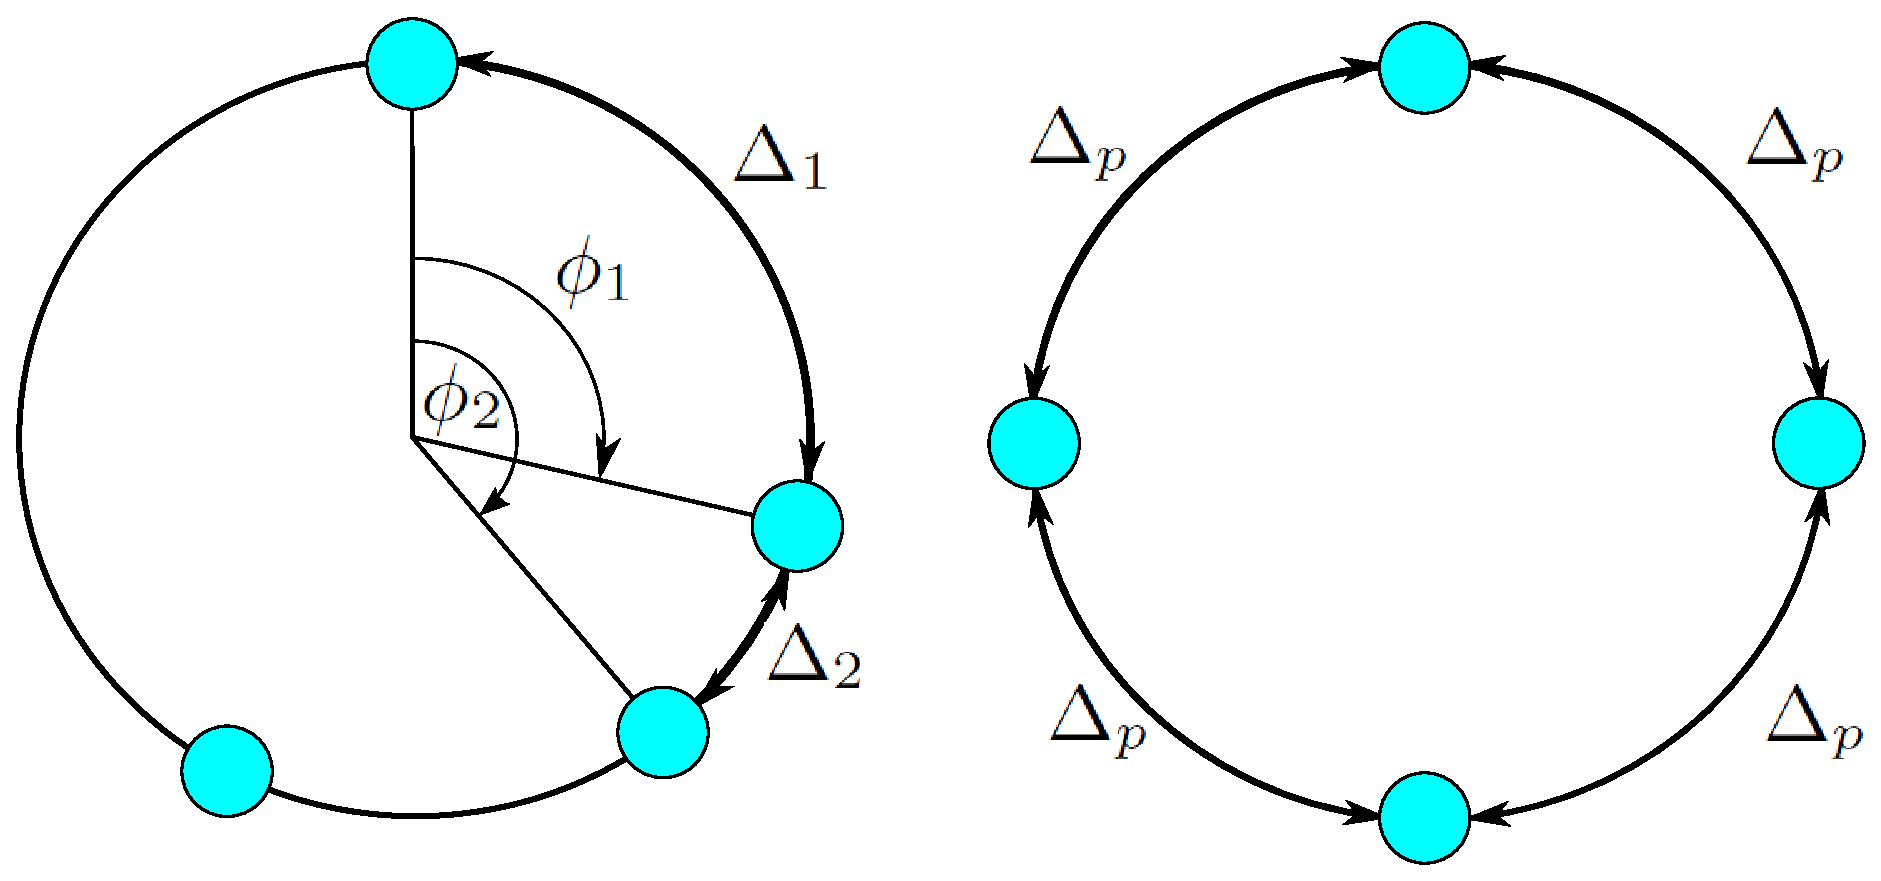
\includegraphics[width=4.0in]{figure/time_circle}
\caption{Desynchronization framework}
\label{fig:time_circle}
\end{figure}

We define terms used in the desynchronization context as follows:

\begin{defn}[Phase]
A phase $\phi_i$ of node $i$ is the time position on the circle of a time period $T$, where $0 \leq \phi_i <  T$ and $T \in \mathbb{R}^+$.
\end{defn}

\begin{defn}[Phase Neighbor]
Node $j$ is a phase neighbor of node $i$ if node $i$ perceives the existence of node $j$ at the phase $\phi_i + \phi_{i,j}$, where $\phi_{i,j}$ is the phase difference between node $j$ and node $i$,
\begin{equation}
\phi_{i,j} = \left\{ 
\begin{array}{l l}
  \phi_j - \phi_i & \quad \mbox{if $\phi_j \geq \phi_i$,}\\
  T - (\phi_i - \phi_j) & \quad \mbox{if $\phi_j < \phi_i$.}\\ \end{array} \right. 
\end{equation}
\end{defn}

\begin{defn}[Next Phase Neighbor]
Node $j$ is the next phase neighbor of node $i$ if $\phi_{i,j} = \min_{k \in S}\{\phi_{i,k}\}$, where $S$ is a set of node $i$'s neighbors. 
%Node $j$ is the next phase neighbor of node $i$ if it has the minimum phase difference among node $i$'s phase neighbors . 
\end{defn}
\begin{defn}[Previous Phase Neighbor]
Node $j$ is the previous phase neighbor of node $i$ if $\phi_{i,j} = \max_{k \in S}\{\phi_{i,k}\}$, where $S$ is a set of node $i$'s neighbors.
%A node $j$ is the next phase neighbor of a node $i$ if it has the maximum phase difference among node $i$'s phase neighbors . 
\end{defn}
\begin{defn}[Desynchrony State]
The system is in the desynchrony state if $\phi_i \neq \phi_j$ for all $i, j \in V$ and  $i \neq j$, where $V$ is a set of nodes in a network that cannot share the same phase.
\end{defn}
\begin{defn}[Perfect Desynchrony State]
The system is in the perfect desynchrony state if it is in the desynchrony state and $\phi_{i,j} = T/N$ for all $i \in V$, $j$ is $i$'s previous phase neighbor, and $N$ is the number of nodes in a network that cannot share the same phase.
\end{defn}

We note that two nodes can share the same phase if they are not within the two-hop communication range of each other.

\section{Related Work}
\label{sec:related}
In this section, we review works in literature. We divide related works into two categories.
The first category is the works on desynchronization in a temporal domain.
The works in this category directly attempt to solve the desynchronization problem in wireless networks.
We compare our work directly to these previous works.
The second category is the works on robotic circular formation. The works in this category do not explicitly attempt to solve the desynchronization problem in wireless networks. However, their works can be abstracted as desynchronization on a spatial domain. These works are the motivation of our desynchronization algorithm.

\subsection{Desynchronization on a Temporal Domain in Wireless Networks}
\label{sec:timedesync}
To the best of our knowledge, DESYNC (\cite{4379660})  is the first to introduce the desynchronization problem. In DESYNC, a node simply attempts to stay in the middle between its previous and next phase neighbors. By repeating this simple algorithm, all nodes will eventually be spread out. However, the error from one phase neighbor is also propagated to the other phase neighbors and indefinitely circulated inside the network. Therefore, DESYNC's error is quite high even after convergence. In contrast, our work relies on all received neighbors information that is robust to the error from one phase neighbor. 
 In  \cite{4663417}, they describe how DESYNC works on multi-hop networks and describe a future extension for DESYNC by exchanging 2-hop neighbors information. 

Designed to converge faster than DESYNC, INVERSE-MS (\cite{4274893}) is an inverse algorithm of the synchronicity work by \cite{MS1990}. 
At a steady state, INVERSE-MS maintains a dynamic equilibrium (\textit{i.e.}, nodes keep changing time positions while maintaining desynchronization). 
However, in INVERSE-MS, the time period is distorted whereas our algorithm does not distort the time period.

In EXTENDED-DESYNC (\cite{MK09DESYNC}), they propose a desynchronization algorithm that is similar to the extension proposed in \cite{4663417}.
Each node sends its one-hop neighbors' relative time information to all of its one-hop neighbors.
Then, the one-hop neighbors relay such information to two-hop neighbors.
Therefore, each node knows 2-hop relative time information.
Consequently, each node can presume that there are two-hop neighbors appearing on the time circle.
Then, each node uses time information of both one-hop and two-hop neighbors and processes with the same algorithm as in DESYNC. Our multi-hop algorithm is partly based on the same idea.

M-DESYNC (\cite{5062256}) is a localized multi-hop desynchronization algorithm that works on a granularity of time slots. The protocol estimates the required number of time slots with a two-hop maximum degree. This estimation helps M-DESYNC converge very fast. However, M-DESYNC requires that all nodes have a global notion of time in order to share the common perception of time slots. Furthermore, M-DESYNC is claimed to work only on acyclic graph networks. On the contrary, our algorithm does not require a global notion of time and can work on both acyclic and cyclic graph networks.

\cite{5062165} propose a simple, lightweight desynchronization algorithm that is also based on a graph coloring model. Unlike M-DESYNC, the algorithm works on general graph networks and does not need the global time. To ensure that the selected time slot does not overlap with others', a node needs to listen to the media for a full time period before claiming the slot. The listening mechanism can only avoid collision with one-hop neighbors but cannot avoid collision with two-hops neighbors (\textit{i.e.}, the hidden terminal problem).
Furthermore, without a common notion of time, the starting time of each slot is quite random. As a result, several time gaps are too small to be used as time slots. This external fragmentation problem reduces resource utilization of the system. Finally, to converge faster, their algorithm overestimates the number of required time slots. Hence, several big time gaps are also left unused and the resource utilization is undoubtedly low. In our work, nodes gradually adapt their phases to be separated from each other as far as possible. Therefore, the external fragmentation problem is reduced. In addition, our algorithm works well on multi-hop networks; each node can avoid collision with two-hops neighbors.

In DESYNC-ORT (\cite{desyncort}), they propose an Orthodontics-inspired desynchronization
algorithm.
In their work, they use information from all one-hop neighbors and attempt to find nodes that are already in corrected time positions and tie them up together.
This method is similar to the Orthodontics method that attempts to tie teeth which are already in corrected positions together.
Their result is better than DESYNC in the term of desynchronization error. 
However, to calculate the correct positions, each node requires to know the total number of nodes in the system in advance. Additionally, the algorithm does not propose to solve the problem in multi-hop networks because nodes in two-hop neighbors can not be tied together with one-hop neighbors. In contrast, our algorithm does not require the total number of nodes in advance. Our algorithm can gradually adapt based on the current number of two-hop neighbors. Additionaly, our algorithm works on multi-hop networks. 

Recently, V-DESYNC (\cite{v-desync}) has been proposed to desynchronize nodes in vehicular ad-hoc networks. Their work has a different objective. They do not focus on fairness (\textit{i.e.}, nodes are not necessary to be equitably separated) because vehicular networks are highly dynamic. In our work, we focus in static wireless sensor networks and attempt to leverage fairness among sensor nodes in resource utilization.

Table \ref{tab:compare} summarizes the advantages and disadvantages of works in this category. The overhead of the proposed algorithm depends on whether the algorithm works on single-hop or multi-hop mode.

\begin{table}
\centering
\begin{tabular}{|c|c|c|c|c|c|c|c|c|} 
\hline
 & \multicolumn{8} {|c|}{Properties} \\  \cline{2-9}
Approach & Period & Time & Equita- & Multi- &  Conver- & Error & Scala- & Over- \\ 
 &  & Synced & ble &  hop	 & gence &  & ble & head \\ 
  &  &  & Spaced  &   &  &  &  &  \\ 
\hline \hline 
DESYNC & Fixed & No & Yes & No & Moderate & High & Poor & Zero  \\ 
  &  &  &  &   &  &  &  &  \\ 
\hline 
INVERSE-MS & Distorted & No & Yes  & No & Fast & Low & Good & Zero \\ 
  &  &  &  &   &  &  &  &  \\ 
\hline 
EXTENDED- & Fixed & No & Yes &  Yes & Moderate & High &  Poor & High \\ 
DESYNC &  &  &  &   &  &  &  &  \\ 
\hline 
M-DESYNC & Fixed & Required & No & Yes & Fast & High & Good & Low \\ 
  &  &  &  &   &  &  &  & \\ 
\hline 
LIGHT-  & Fixed & No & No & Yes & Fast & High & Good & Zero \\ 
WEIGHT &  &  &  &   &  &  &  & \\ 
\hline 
DESYNC-  & Fixed & No & Yes & No & Moderate & Low & Good & Zero \\ 
ORT &  &  &  &   &  &  &  & \\ 
\hline 
V-DESYNC  & Fixed & No & No & No & No & High & Good & Zero \\ 
  &  &  &  &   &  &  &  &  \\ 
\hline 
Proposed & Fixed & No & Yes & Yes & Moderate & Low &  Good & Zero/ \\ 
  &  &  &  &   &  &  &  & Low \\ 
\hline 
\end{tabular} 
\caption{Desynchronization Protocols Comparison}
\label{tab:compare}
\end{table}

\subsection{Desynchronization on a Spatial Domain in Robotics}
\label{sec:spacedesync}
In robotic pattern formation, multiple robots distributedly group and align themselves in geometric patterns such as circle, rectangle, and triangle. Without an explicit argument, robotic pattern formation can be abstracted as desynchronization on a spatial domain. Robots attempt to separate away from each other as far as possible to form such patterns. In other words, robots desynchronize themselves spatially to avoid the collision with each other in the spatial domain.

Several works have done in several pattern formations (\cite{suzuki-96}, \cite{suzuki-99}). However, the pattern formation that is similar to desynchronization on the temporal domain is the formation on a closed ring. 
Figure \ref{fig:robotic-closed-ring} illustrates the robotic formation on a closed ring. In Figure \ref{fig:closedring}, initially, robots are randomly placed on any position on the closed ring. The perfect configuration of the formation is illustrated in Figure \ref{fig:closedring-perfect}. Robots are equivalently separated away on the ring. 

\begin{figure*}[!t]
\centerline {
	\subfloat[]{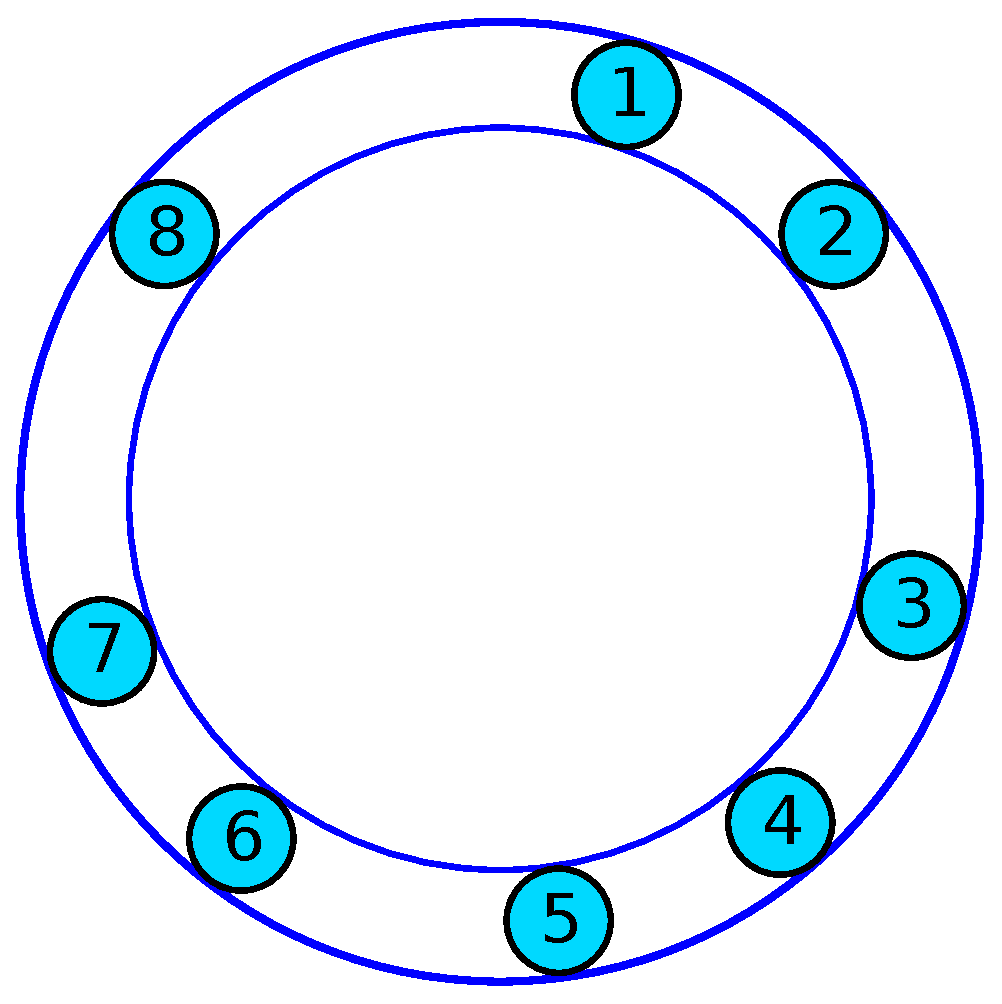
\includegraphics[width=2in]{figure/robotic-closed-ring}%
	\label{fig:closedring}}
	\hfil
	\subfloat[]{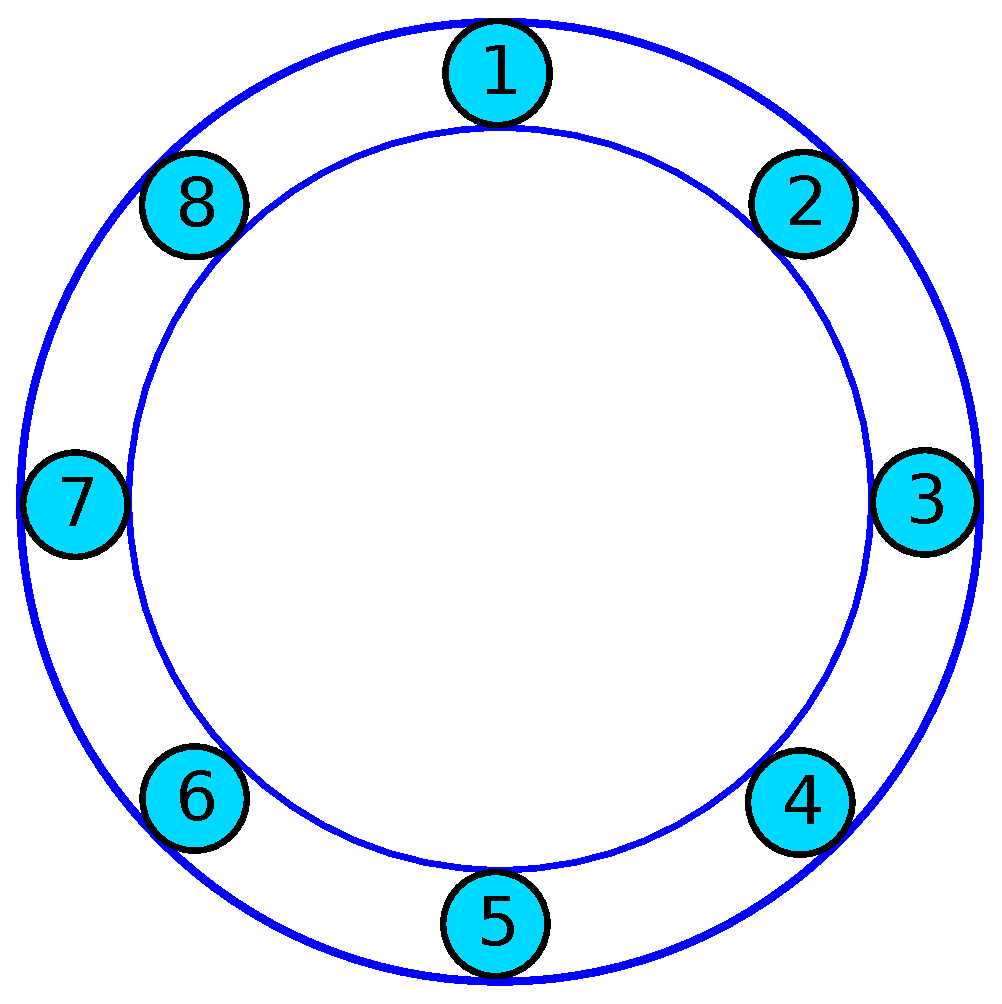
\includegraphics[width=2in]{figure/robotic-closed-ring-perfect}%
	\label{fig:closedring-perfect}}
}
\caption{Robotic pattern formation on a closed ring. (a) Robots are randomly placed on a closed ring. (b) In the perfect configuration, robots are equitably separated from each other. }
\label{fig:robotic-closed-ring}
\lofcont
\end{figure*}

Several previous works such as \cite{defago04}, \cite{cohen-08}, and \cite{flocchini-08} have proposed algorithms that are similar to each other for robotic formation on a closed ring. These works assume robots have limited visibility range. Each robot attempts to adjust its position to the middle between two nearest robots on its left side and right side (Figure \ref{fig:closedring-desync}). In these works, they prove that this simple algorithm eventually converges to the perfect configuration (Figure \ref{fig:closedring-desync-perfect}).

\begin{figure*}[!t]
\centerline {
	\subfloat[]{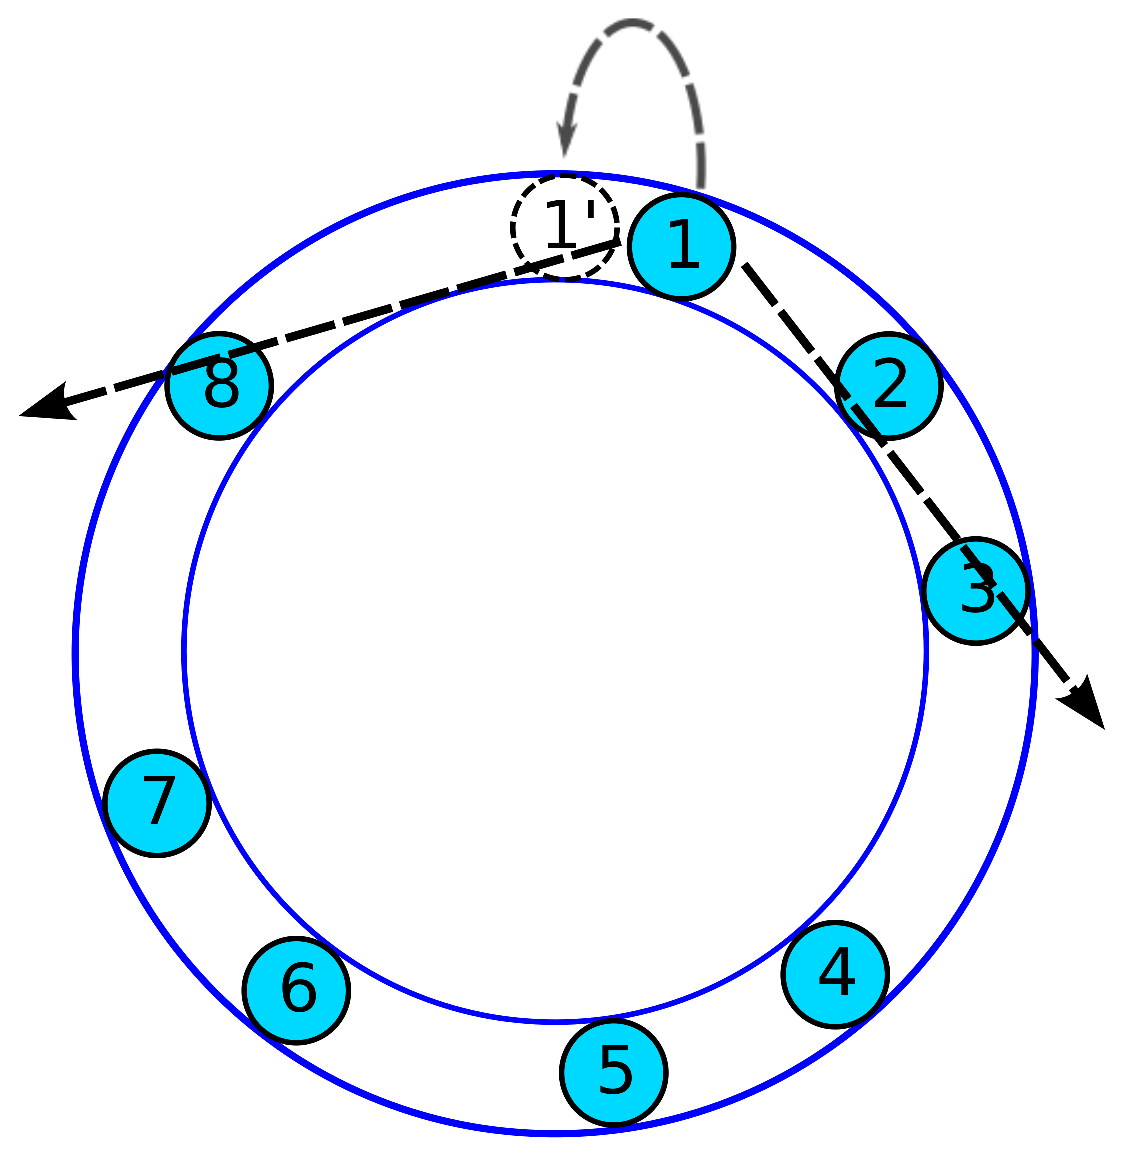
\includegraphics[width=2in]{figure/robotic-closed-ring-desync}%
	\label{fig:closedring-desync}}	
	\hfil
	\subfloat[]{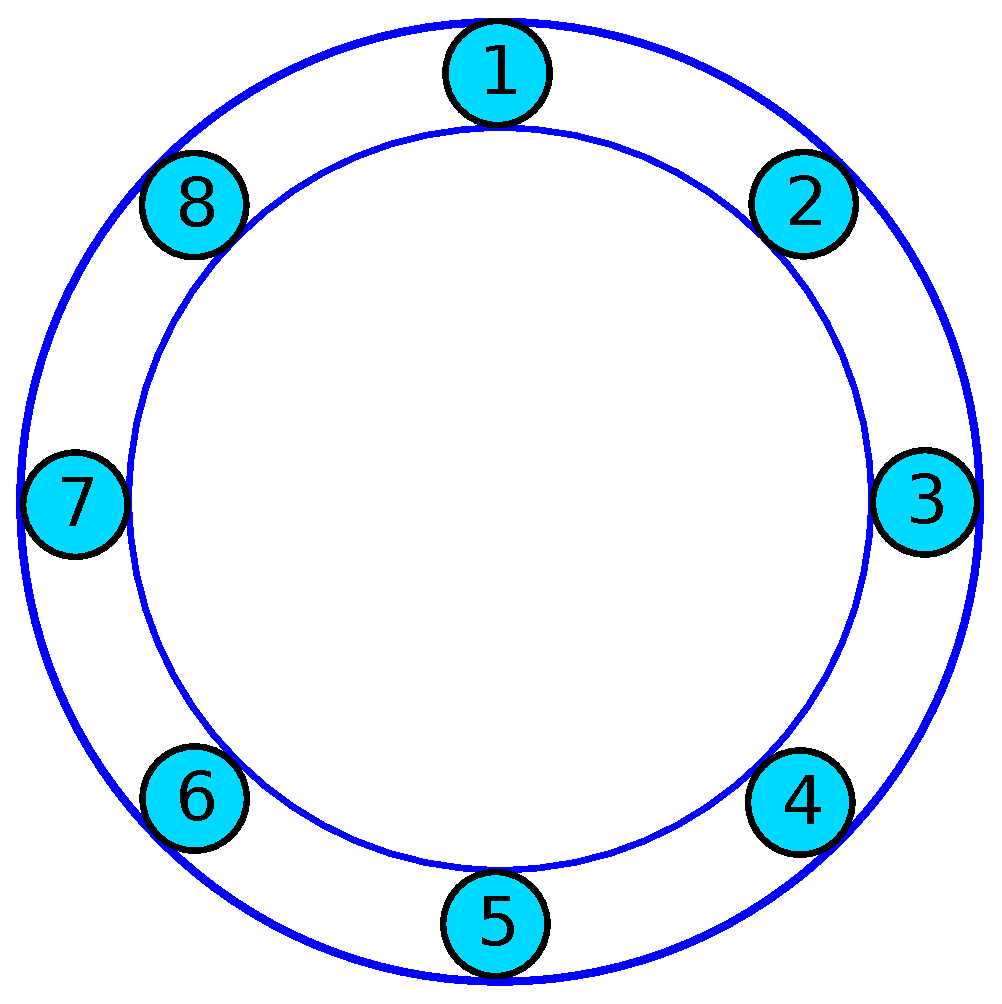
\includegraphics[width=2in]{figure/robotic-closed-ring-desync-perfect}%
	\label{fig:closedring-desync-perfect}}	
}
\caption{Moving to the midpoint algorithm. (a) Each robot moves to the midpoint between two nearest visible neighbors. (b) The algorithm converges to the perfect configuration.}
\label{fig:robotic-closed-ring-desync}
\lofcont
\end{figure*}

In \cite{4141997}, heterogeneous robots are distributedly grouped into teams that are equally spread out to cover the monitored area. Each robot has no global knowledge of others’ absolute positions but can detect relative positions of the others with respect to itself as well as the type of the others. 
To form a circle, an artificial force is used as an abstraction for velocity adaptation of a robot. 
Robots of different types have attracting forces to each other. Conversely, robots of the same type have repelling forces. As a result, the circle of heterogeneous robots will be formed and robots are nicely spaced on the circle  (see Figure \ref{fig:circular_formation}). This work inspires our desynchronization algorithm.

\begin{figure}[!t]
\centering
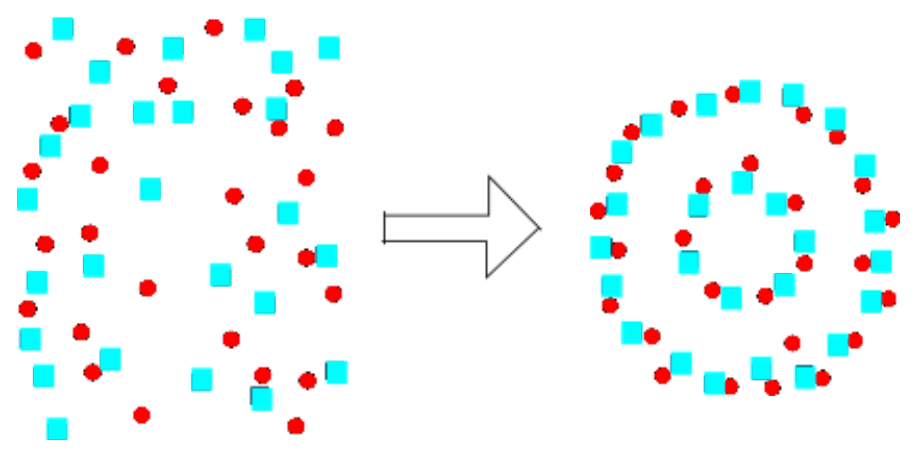
\includegraphics[width=5.0in]{figure/robo_new}
\caption{Results of Robotic Circular Formation. Robots with two different types form the circle.}
\label{fig:circular_formation}
\end{figure}

\subsection{Others}
\label{sec:tdma}
Other works that are related to desynchronization protocols are distributed Time Division Multiple Access (TDMA) protocols. Distributed TDMA protocols are similar to M-DESYNC (\cite{5062256}); their protocols work on a granularity of time slots. 
As same as M-DESYNC, most of distributed TDMA protocols such as TRAMA (\cite{trama}), Parthasarathy \cite{Parthasarathy}, ED-TDMA (\cite{edtdma}), and Herman (\cite{herman}) assume time is already slotted or all nodes are synchronized to achieve the same global clock. 
%Some distributed TDMA protocols do not require time synchronization. However, they require more states and incur control message overhead. For example, DRAND \cite{4803842}  requires the control overhead for sending request, reject, release, and grant messages. 
In our work, we do not require time synchronization and do not assume already slotted time.

\section{Motivation}
\label{sec:motivation}
We observe that the desynchronization framework on the temporal domain is similar to the robotic circular formation which can be abstracted as the desynchronization on the spatial domain.
In the desynchronization framework on the temporal domain, a node (like a robot) does not have a global notion of time but each node can measure relative time differences with other nodes.
The circle of robots is similar to our circle of the time period. 
The distribution of robots can be mapped to the distribution of nodes on the time circle. 
The robotic circular formation of \cite{4141997} inspires us to design a novel desynchronization algorithm for wireless sensor networks based on an \textit{artificial force field}.
If we abstract the nodes on a time circle as the robots of the same type, the nodes will repel each other and keep time intervals from their neighbors as far as possible.
Once all received forces are balanced, nodes are equally spread out on the time circle.

The desynchronization algorithm based on the artificial force field can be classified as a \textit{Physicomimetics} algorithm.
A physicomimetics algorithm is an algorithm that imitates principles of physics and can be called \textit{Artificial Physics} or \textit{Virtual Physics} (\cite{physicomimetics}). To the best of our knowledge, physicomimetics was introduced in \cite{810278} for distributed control of large collections of agents. Then, physicomimetics has been applied mostly in the field of robotics for geometric pattern formation and optimizations such as in \cite{swarm}, \cite{artphysics}, and \cite{4141997}.
Due to the framework of desynchronization is similar to the framework of robotic geometric pattern formation, we believe that the physicomimetics approach can also solve the desynchronization problem in the temporal domain as well. 
Therefore, this dissertation presents how physics principles can be imitated to solve the desynchronization problem for wireless sensor networks.
